% 104-100(104쪽) — 대각선의 길이가 6인 직육면체(앞면 왼쪽 위 꼭짓점에서 뒷면 오른쪽 아래 꼭짓점으로 그은 대각선).
% 스캔 화질이 낮아 TikZ 로 다시 그림. 라벨은 원문 그대로 대각선의 6 만 두고
% 모서리의 길이·합(답)은 그림에 나타내지 않는다.
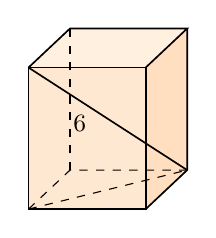
\begin{tikzpicture}[scale=0.62, line width=0.6pt]
  \coordinate (FBL) at (0,0); \coordinate (FBR) at (2.4,0);
  \coordinate (FTR) at (2.4,2.9); \coordinate (FTL) at (0,2.9);
  \coordinate (BBL) at (0.85,0.8); \coordinate (BBR) at (3.25,0.8);
  \coordinate (BTR) at (3.25,3.7); \coordinate (BTL) at (0.85,3.7);
  \fill[orange!18] (FBL) -- (FBR) -- (FTR) -- (FTL) -- cycle;
  \fill[orange!12] (FTL) -- (BTL) -- (BTR) -- (FTR) -- cycle;
  \fill[orange!25] (FBR) -- (BBR) -- (BTR) -- (FTR) -- cycle;
  \draw (FBL) -- (FBR) -- (FTR) -- (FTL) -- cycle;
  \draw (FTL) -- (BTL) -- (BTR) -- (FTR);
  \draw (FBR) -- (BBR) -- (BTR);
  \draw[dashed, line width=0.4pt] (FBL) -- (BBL) -- (BBR);
  \draw[dashed, line width=0.4pt] (BBL) -- (BTL);
  \draw[dashed, line width=0.4pt] (FBL) -- (BBR);
  \draw[line width=0.6pt] (FTL) -- (BBR);
  \node[font=\small] at (1.05,1.75) {$6$};
\end{tikzpicture}
